\documentclass[a4paper,12pt]{report}

\usepackage{tikz}
\usetikzlibrary{shapes,arrows,chains, trees}

\title{Computing Practical Project Diagrams}
\author{Oscar Daniel}
\date{Febuary 2015 }
\begin{document}



\begin{tikzpicture}
\draw [->] (0,0) -- (2,0);

\end{tikzpicture}

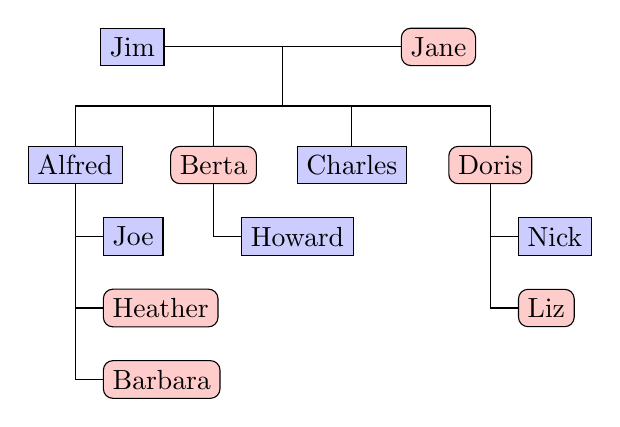
\begin{tikzpicture}[
  man/.style={rectangle,draw,fill=blue!20},
  woman/.style={rectangle,draw,fill=red!20,rounded corners=.8ex},
  grandchild/.style={grow=down,xshift=1em,anchor=west,
    edge from parent path={(\tikzparentnode.south) |- (\tikzchildnode.west)}},
  first/.style={level distance=6ex},
  second/.style={level distance=12ex},
  third/.style={level distance=18ex},
  level 1/.style={sibling distance=5em}]
    % Parents
    \coordinate
      child[grow=left] {node[man,anchor=east]{Jim}}
      child[grow=right] {node[woman,anchor=west]{Jane}}
      child[grow=down,level distance=0ex]
    [edge from parent fork down]
    % Children and grandchildren
    child{node[man] {Alfred}
      child[grandchild,first] {node[man]{Joe}}
      child[grandchild,second] {node[woman]{Heather}}
      child[grandchild,third] {node[woman] {Barbara}}}
    child{node[woman] {Berta}
      child[grandchild,first] {node[man]{Howard}}}
    child {node[man] {Charles}}
    child {node[woman]{Doris}
      child[grandchild,first] {node[man]{Nick}}
      child[grandchild,second] {node[woman]{Liz}}};
\end{tikzpicture}
\end{document}